% Especificaciones del tamaño de letra, tamaño de hoja, márgenes, librerias, etc.
\documentclass[12pt, letterpaper]{article}
\usepackage[english]{babel}
\usepackage[utf8]{inputenc}
\usepackage[T1]{fontenc}
\usepackage{mathrsfs}
\usepackage{amsmath}
\usepackage{graphicx}
\usepackage{subcaption}
\usepackage{hyperref}
\usepackage{url}
\usepackage{amssymb}
\usepackage{float}
\usepackage[margin=1in]{geometry}
\renewcommand{\baselinestretch}{1.5}

% Enlace Bibliografía
\usepackage{csquotes}
\usepackage[notes,backend=biber]{biblatex-chicago}
\addbibresource{referencias.bib}

% Titulo, autores, fecha.
\title{Tarea \#3: Termoeconomía}
\author{Carlos Vásquez 1155057}

% Inicio del documento
\begin{document}
\maketitle
\section*{Introducción}

Dada la preocupación creciente por el ahorro de energía, se ha fomentado el desarrollo de técnicas de análisis para optimizar los procesos que llevan a cabo las industrias. Esto nos ha llevado a desarrollar la termoeconomía, la cual es la rama de la ingeniería energética que, mediante la aplicación combinada del análisis termodinámico y el análisis económico, permite lograr resultados que no se obtendrían mediante el análisis por separado que brindarían estas disciplinas. \autocite{montes09}

Los conceptos que principalmente oscilan en esta disciplina son los de exergía y el de la segunda ley de la termodinámica, así como los costes económicos de los recursos y productos que intervienen en los procesos industriales. 

\section*{Objetivos}

Las fuentes energéticas primarias, es decir, las disponibles en la naturaleza como los combustibles fósiles, , energía eólica, energía solar, energía hidráulica, etc., en principio se consideran inagotables, a excepción de los combustibles fósiles que se limitan a las reservas mundiales. El mundo es en gran parte dependiente del carbón, petróleo y gas natural, que son limitados y aún así el consumo mundial de fuentes de energía para estos combustibles es del 85\%. Ello conduce a una reflexión sobre el consumo de energía y cómo aprovecharla de mejor manera, proporcionando una motivación más para el análisis termoeconómico que se puede realizar.\autocite{silva15}

La termoeconomía proporciona una herramienta muy potente y rigurosa para lograr el análisis y la optimización de procesos industriales, y así lograr reducir los \textit{costes de energía}. Toda máquina que no tenga una buena eficiencia nos proporcionará una mayor cantidad de pérdidas en energía, lo cual se traduce a costo monetario, ya sea en equipos para depurar los residuos que éstas producen, necesidad de más combustible, etcétera. Esto nos reafirma que las \textit{energías limpias} tienen que ser eficientes, dado que la generación de residuos disminuye su estándar de limpieza.

Cuando de un sistema se obtiene solamente un producto, el coste de producción de éste será la suma de los costes originados y se calcula con un \textit{balance de costes}, análogo al balance de energías con el que se lidia en termodinámica tradicional. Sin embargo, sería absurdo determinar los costes a partir de las energías proporcionadas por la transferencia de calor y el trabajo que se realice , lo correcto sería asignar los costes en proporción de las \textit{exergías}, que reflejan adecuadamente sus respectivos efectos útiles. \autocite{montes09}

En general, la termoeconomía tiene los siguientes objetivos:

\begin{itemize}
	\item Calcular los costes de los productos intermedios y finales de los procesos.
	\item Analizar el proceso de formación y el flujo de los costes en los procesos.
	\item Valorar el coste de las destrucciones y pérdidas de exergía.
	\item Optimizar el funcionamiento de cada componente de un sistem y el de éste en su conjunto.
	\item Optimizar el coste de los productos de un sistema.
\end{itemize}

\section*{Aplicaciones}

Anteriormente hemos hablado de los objetivos de la termoeconomía y queda muy claro que su gama de aplicaciones es muy amplia. En general, cualquier proceso que se analice tiene probabilidades de ser optimizado, no obstante, la evaluación final de cualquier proceso debe realizarse en términos monetarios incorporando al coste de los flujos internos y productos todos y cada uno de los recursos utilizados. Dejando de lado la perspectiva puramente física del coste del producto, también entran en juego el ambiente económico caracterizado por el precio del mercado de las fuentes de energía. A pesar del capital con el que contemos para realizar nuestros procesos, podemos reducir en gran parte los costes si la estructura del sistema y la calidad del funcionamiento de los equipos son las óptimas. Claro esta que, si tomamos en cuenta los costes de capital, tendremos que minimizar el coste unitario de producto, en el cual se consideran tanto las variables físicas como las variables económicas del mercado actual.\autocite{lozano97}

Habiendo dicho todo lo anterior, en general las aplicaciones de la termoeconomía son en un sector industrial, en donde se necesite cotizar aquellos costos que involucra la implementación de un sistema o proceso. También se utiliza para hallar optimizaciones en un proceso y volverlo más eficiente. En otras ocasiones se ha utilizado para mejorar el ahorro de energía de algunos dispositivos. Ejemplos muy claros surgen en la ecología industrial, en donde se ha implementado para transformar procesos industriales lineales en sistemas de circuito cerrado, haciendo que éstos se asemejen a procesos que ocurren en los ecosistemas naturales y volviéndolos más sostenibles, en lo que el tratamiento de residuos se m aneja de manera eficiente y rentable.
\subsection*{Ejemplo de Análisis Termoeconómico}
Para ilustrar los puntos anteriores, se recurrirá a un ejemplo sencillo donde se analizará el sigiuiente problema.

Se trata de diseñar una caldera de recuperación de la energía térmica de los gases de escape de una turbina de gas para la producción de vapor saturado a $P_v = 10\ bar$. La turbina de gas ya existe y produce  3000 kW de potencia neta para una pérdida de presión admisible de 0.036 bar para los gases de escape que atravesarán la caldera de recuperación. El flujo másico de los gases de escape que abandonan la turbina a una temperatura $T_g = 864.6\ K$ (591.3 ºC) es de $\dot{m}_g = 9.928\ kg/s$. Se supondrá que el calor específico de los gases es constante e igual a $c_g = 1\ \frac{kJ}{kg K}$. El esquema de instalación se muestra a continuación:

\begin{figure}[H]
	\centering
	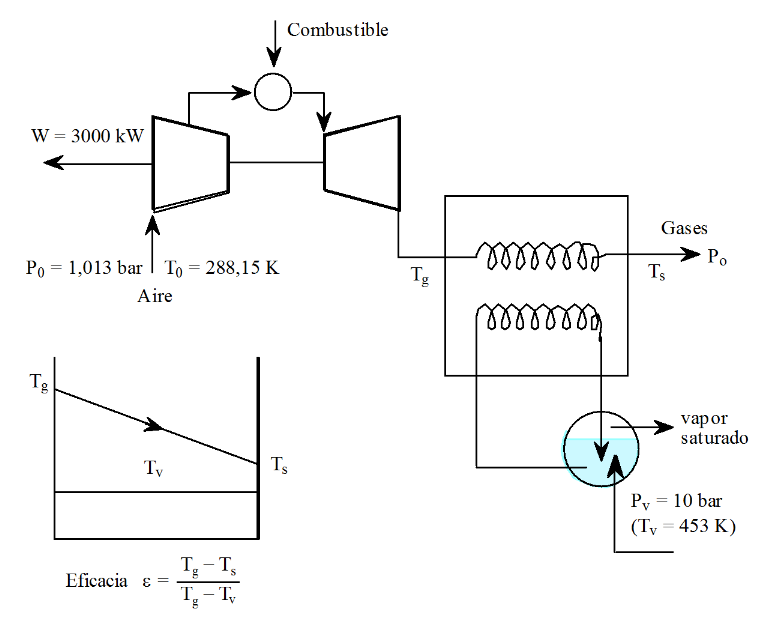
\includegraphics[width=0.9\textwidth]{sys.png}
	\caption{Esquema de la caldera de recuperación. Obtenido de \textit{"Aplicaciones Termoeconómicas del Método Exergético" por Lozano Serrano, M. A. (1997), pg. 17}}
\end{figure}

En las condiciones descritas la inversión a realizar en la caldera de recuperación depende de su eficacia

\begin{equation}
	J = 1610 \dot{m}_g \log{\frac{1}{1-\varepsilon}} \ \ \ \ (\$)
\end{equation}

El flujo de calor máximo que puede recuperarse en la caldera se obtiene para $\varepsilon = 1$, lo que implica $T_s = T_v$ y una superficie de intercambio de calor infinita. Por tanto:

\begin{equation}
	\dot{Q}_{max} = \dot{m}_g c_g (T_g - T_v) = 4083\ kW
\end{equation}

Este equivale a una cantidad de producto expresado en energía

\begin{equation}
	P_{max} = \dot{Q}_{max}\bigg(1 - \frac{T_0}{T_v}\bigg) = 1483\ kW
\end{equation}

La exergía térmica de los gases (fuel) es la siguiente:

\begin{equation}
	F = \dot{m}_g c_g \Bigg(T_g - T_0 - T_0\log{\frac{T_g}{T_0}}\Bigg) = 2578\ kW
\end{equation}

Y por tanto, el rendimiento exergético máximo resulta

\begin{equation}
	\eta_{max} = \frac{P_{max}}{F} = 0.5765
\end{equation}

Para un determinado valor de eficacia $\varepsilon$ el rendimiento exergético podrá calcularse como $\eta = \varepsilon \cdot \eta_{max}$. Suponiendo un factor de amortización $\xi = 6.7 \times 10^{-9} s^{-1}$, calculando la inversión necesaria J ($\varepsilon$) con la ecuación suministrada y realizando un ajuste de los resultados a la fórmula:

\begin{equation}
	Z = \xi \alpha \Bigg(\frac{1}{\eta_{max} - \eta} \Bigg)^n F^m
\end{equation}

Para $0.95 < \varepsilon < 0.995$ se obtienen los siguientes coeficientes:

\begin{equation}
	\begin{split}
		\xi \alpha &= 5.95 \times 10^{-8}\ \frac{\$}{kJ}\\
		n &= 0.318\\
		m &= 1
	\end{split}
\end{equation}

Aplicando las condiciones de optimidad obtenidas antes para distintos escenarios relativos al coste de producción de la exergía del vapor por medios convencionales resulta:

\begin{figure}[H]
	\centering
	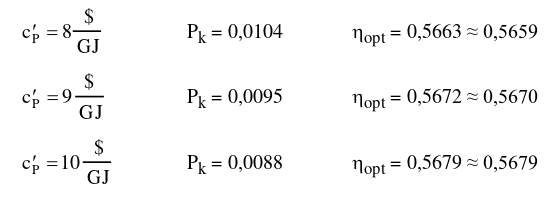
\includegraphics[width=0.7\textwidth]{table.png}
\end{figure}

donde los valores a la derecha corresponden al óptimo real.

Detallando los resultados para el último caso:
\begin{equation}
	\begin{split}
		\varepsilon = \frac{\eta}{\eta_{max}} &\approx  0.985\\
		T_s = T_g - \varepsilon (T_g - T_v) &\approx 459\ K\\
		\Delta T_{pinch} = T_s = T_v &\approx 6\ K\\
		\dot{Q} = \varepsilon \dot{Q}_{max} &= 4020\ kW\\
		P = \varepsilon P_{max} &= 1460\ kW\\
		Z = 5.95 \times 10^{-8} \Bigg( \frac{1}{\eta_{max} - \eta}\Bigg)^{0.318} F &= 6.96 \times 10^{-4} \frac{\$}{s}\\
		J = \frac{Z}{\xi} &= 104000\ \$\\
		Ahorro = c_p' P - Z &= 0.014 \frac{\$}{s}
	\end{split}
\end{equation}

\section*{Notas finales}

El ejemplo mostrado fue obtenido del artículo citado previamente, sin embargo es difícil seguir lo que se realiza sin el entendimiento de las fórmulas utilizadas. Gran parte de las fórmulas utilizadas son derivadas en el mismo documento citado, sin embargo gran parte del análsisi termodinámico (exergías, transferencia de calor, etcétera) se asume que el lector lo conoce de antemano. A pesar de esto, las fórmulas utilzadas no son tan complejas, y resultan sencillas de utilizar para encontrar la inversión total a realizar.

%%%%%  Bib
\renewcommand\refname{Referencias}
\printbibliography
\end{document}
